\setcounter{equation}{0}
\question \textgreek{Σωστή απάντηση: $i$}
\begin{proof}[\unskip\nopunct]
\begin{align*}
    &e^\pi > \pi^e\\
    \underset{\mathrm{\pi^e > 0}}{\overset{\mathrm{e^\pi > 0}}{\implies}}& \pi > eln\pi\\
    \implies& \pi - eln\pi > 0
\end{align*}
\begin{center}
\textgreek{Το οποίο ισχύει. Διότι: }
        
\textgreek{Έστω $f(x) = x-elnx$, $x > 0$.}
        
\textgreek{Η $f$ είναι παραγωγήσιμη ως πράξεις παραγωγήσιμων σηναρτήσεων.}
\end{center}
\begin{equation*}
    f'(x) = 1 - \frac{e}{x} = \frac{x-e}{x}, x>0
\end{equation*}
\begin{align*}
    &f'(x) = 0 \implies \frac{x-e}{x} = 0 \implies x = e\\
    &x > e \implies x-e > 0 \overset{x>0}{\implies} \frac{x-e}{x} > 0\\
    &x < e \implies x-e < 0 \overset{x>0}{\implies} \frac{x-e}{x} < 0
\end{align*}

\begin{center}
    \begin{tikzpicture}
        \tkzTabInit[espcl=3]{$x$ /1,$f'(x)$ /1, $f(x)$ /2 }
            {$0$ ,$e$, $\pi$, $+\infty$}
        \tkzTabLine {,-,z,,+ ,  }
        \tkzTabVar{+/,-/, R/, +/}
    \end{tikzpicture}
\end{center}

\begin{center}
\textgreek{Άρα το $f(e)$ είναι (ολικό) ελάχιστο. Οποτέ θα έχουμε ότι: }
\begin{align*}
    &f(\pi) > f(e)\\
    \implies &\pi - eln\pi > e - elne\\
    \implies &\pi - eln\pi > 0
\end{align*}
\end{center}
\end{proof}